\chapter{Konzepte \& Architektur}
\section{Konzepte}
Für die Bewältigung der Anforderungen an die Softwarelösung wurden einige Konzepte entwickelt, welche Einfluss auf die einzelnen Komponenten und die Architektur genommen haben. Die Softwarelösung soll wie unter \ref{ch:anforderungen_section} \nameref{ch:anforderungen_section} beschrieben die Möglichkeit bieten eine Karte darzustellen, auf welcher die Simulationsdaten dargestellt werden und bearbeitet werden können. Die Bearbeitung sollte jedoch keinen Einfluss auf die Stammdaten haben. Diese Konzepte werden in den folgenden Kapiteln beschrieben.
\subsection{Datentiles}
Um die grosse Datenmenge (ca. 2,8 Millionen Datensätze für die Schweiz) zu bewältigen wurde ein bewährtes Verfahren für Kartendarstellung verwendet. Dabei werden die Daten nicht als gesamtes geliefert sondern über Tiles angefragt. Ein Tile ist ein Quadrat welches ein bestimmten Bereich der Welt deckt. Durch die Anforderung eines dieser Quadrate kann sichergestellt werden, dass nicht zu viele Daten auf einmal angefragt werden. Ein weiteres Konzept in Verbindung mit diesem wird unter \ref{sec:concept_preprocessing} \nameref{sec:concept_preprocessing} beschrieben. Dabei werden die Daten für jede Zoomstufe bewertet und nur ausgegeben wenn diese Relevant sind. Durch dieses Konzept kann die Datenmenge die von der Website verarbeitet werden muss stark reduziert werden.
\begin{figure}[H]
\centering
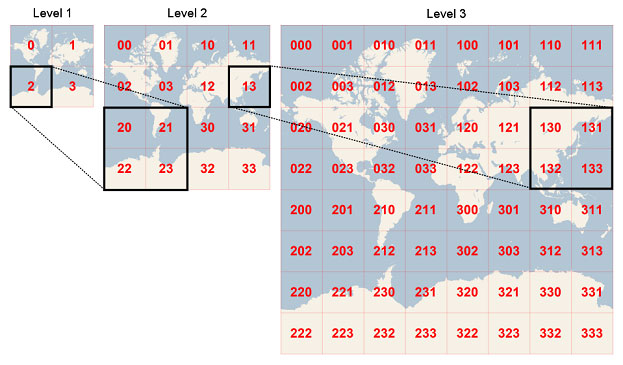
\includegraphics[height=7cm]{images/BingMapsTileSystem.jpg}
Quelle: \href{https://msdn.microsoft.com/en-us/library/bb259689.aspx}{https://msdn.microsoft.com/en-us/library/bb259689.aspx}
\caption{Aufteilung der Welt in Tiles und Berechnung des QuadKey}
\label{fig:tilesystem}
\end{figure}
Um von einem Eintrag auf das Tile zu schliessen, in welchem dieser sichtbar ist, wird ein Schlüssel (QuadKey) berechnet. Der QuadKey benennt eindeutig das kleinstmögliche Tile in welchem der ganze Eintrag (z.B. eine Strasse) angezeigt werden kann. Der QuadKey wird nach dem System in Abbildung \ref{fig:tilesystem} erstellt. Dabei wird auf der äussersten Zoomstufe die Welt in 4 Tiles aufgeteilt. Diese werden nummeriert. z.B. 0 für links oben, 1 für rechts oben. Um die nächste Stufe der Tiles zu erstellen, wird jedes Tile wieder in 4 Tiles aufgeteilt und dann ebenfalls nummeriert. Dabei wird als Prefix die Nummer des alten Tiles verwendet. Dadurch kann jedes Tile auf jeder Zoomstufe eindeutig adressiert werden. Der QuadKey bietet auch die Möglichkeit mit Hilfe des Prefix alle Tiles unterhalb eines Tiles zu berechnen. So starten alle QuadKeys welche auf einer beliebigen Zoomstufe in einem Tile unterhalb des linken oberen Tile auf Level 1 sind mit einer 0. Dieser Ansatz kann für die Filterung der Daten verwendet werden.
\subsection{Preprocessing und Bewertung der Daten}\label{sec:concept_preprocessing}
Um die Zugriffszeiten der Datenbank zu erhöhen werden die Daten beim Importieren vorberechnet. Durch diesen Vorgang werden bewusst Redundanzen in das Datenmodell eingeführt. Diese Redundanzen erlauben den Zugriff auf Daten ohne teure JOIN Statements oder SQL Funktionen aufzurufen. Auf die Vorberechnungen welche im Datenmodell verwendet werden wird tiefer im Abschnitt \ref{sec:tilingdataimplementation} \nameref{sec:tilingdataimplementation} eingegangen. Um weiteren Berechnungsaufwand zu reduzieren wird jeder Datensatz neben der Vorberechnung auf seine Anzeigewichtigkeit bewertet. Dabei wird berechnet ab welcher Stufe z.B. die Strasse dargestellt wird.

\subsection{Changeset}
TODO
\section{Architektur}
\begin{figure}[H]
\centering
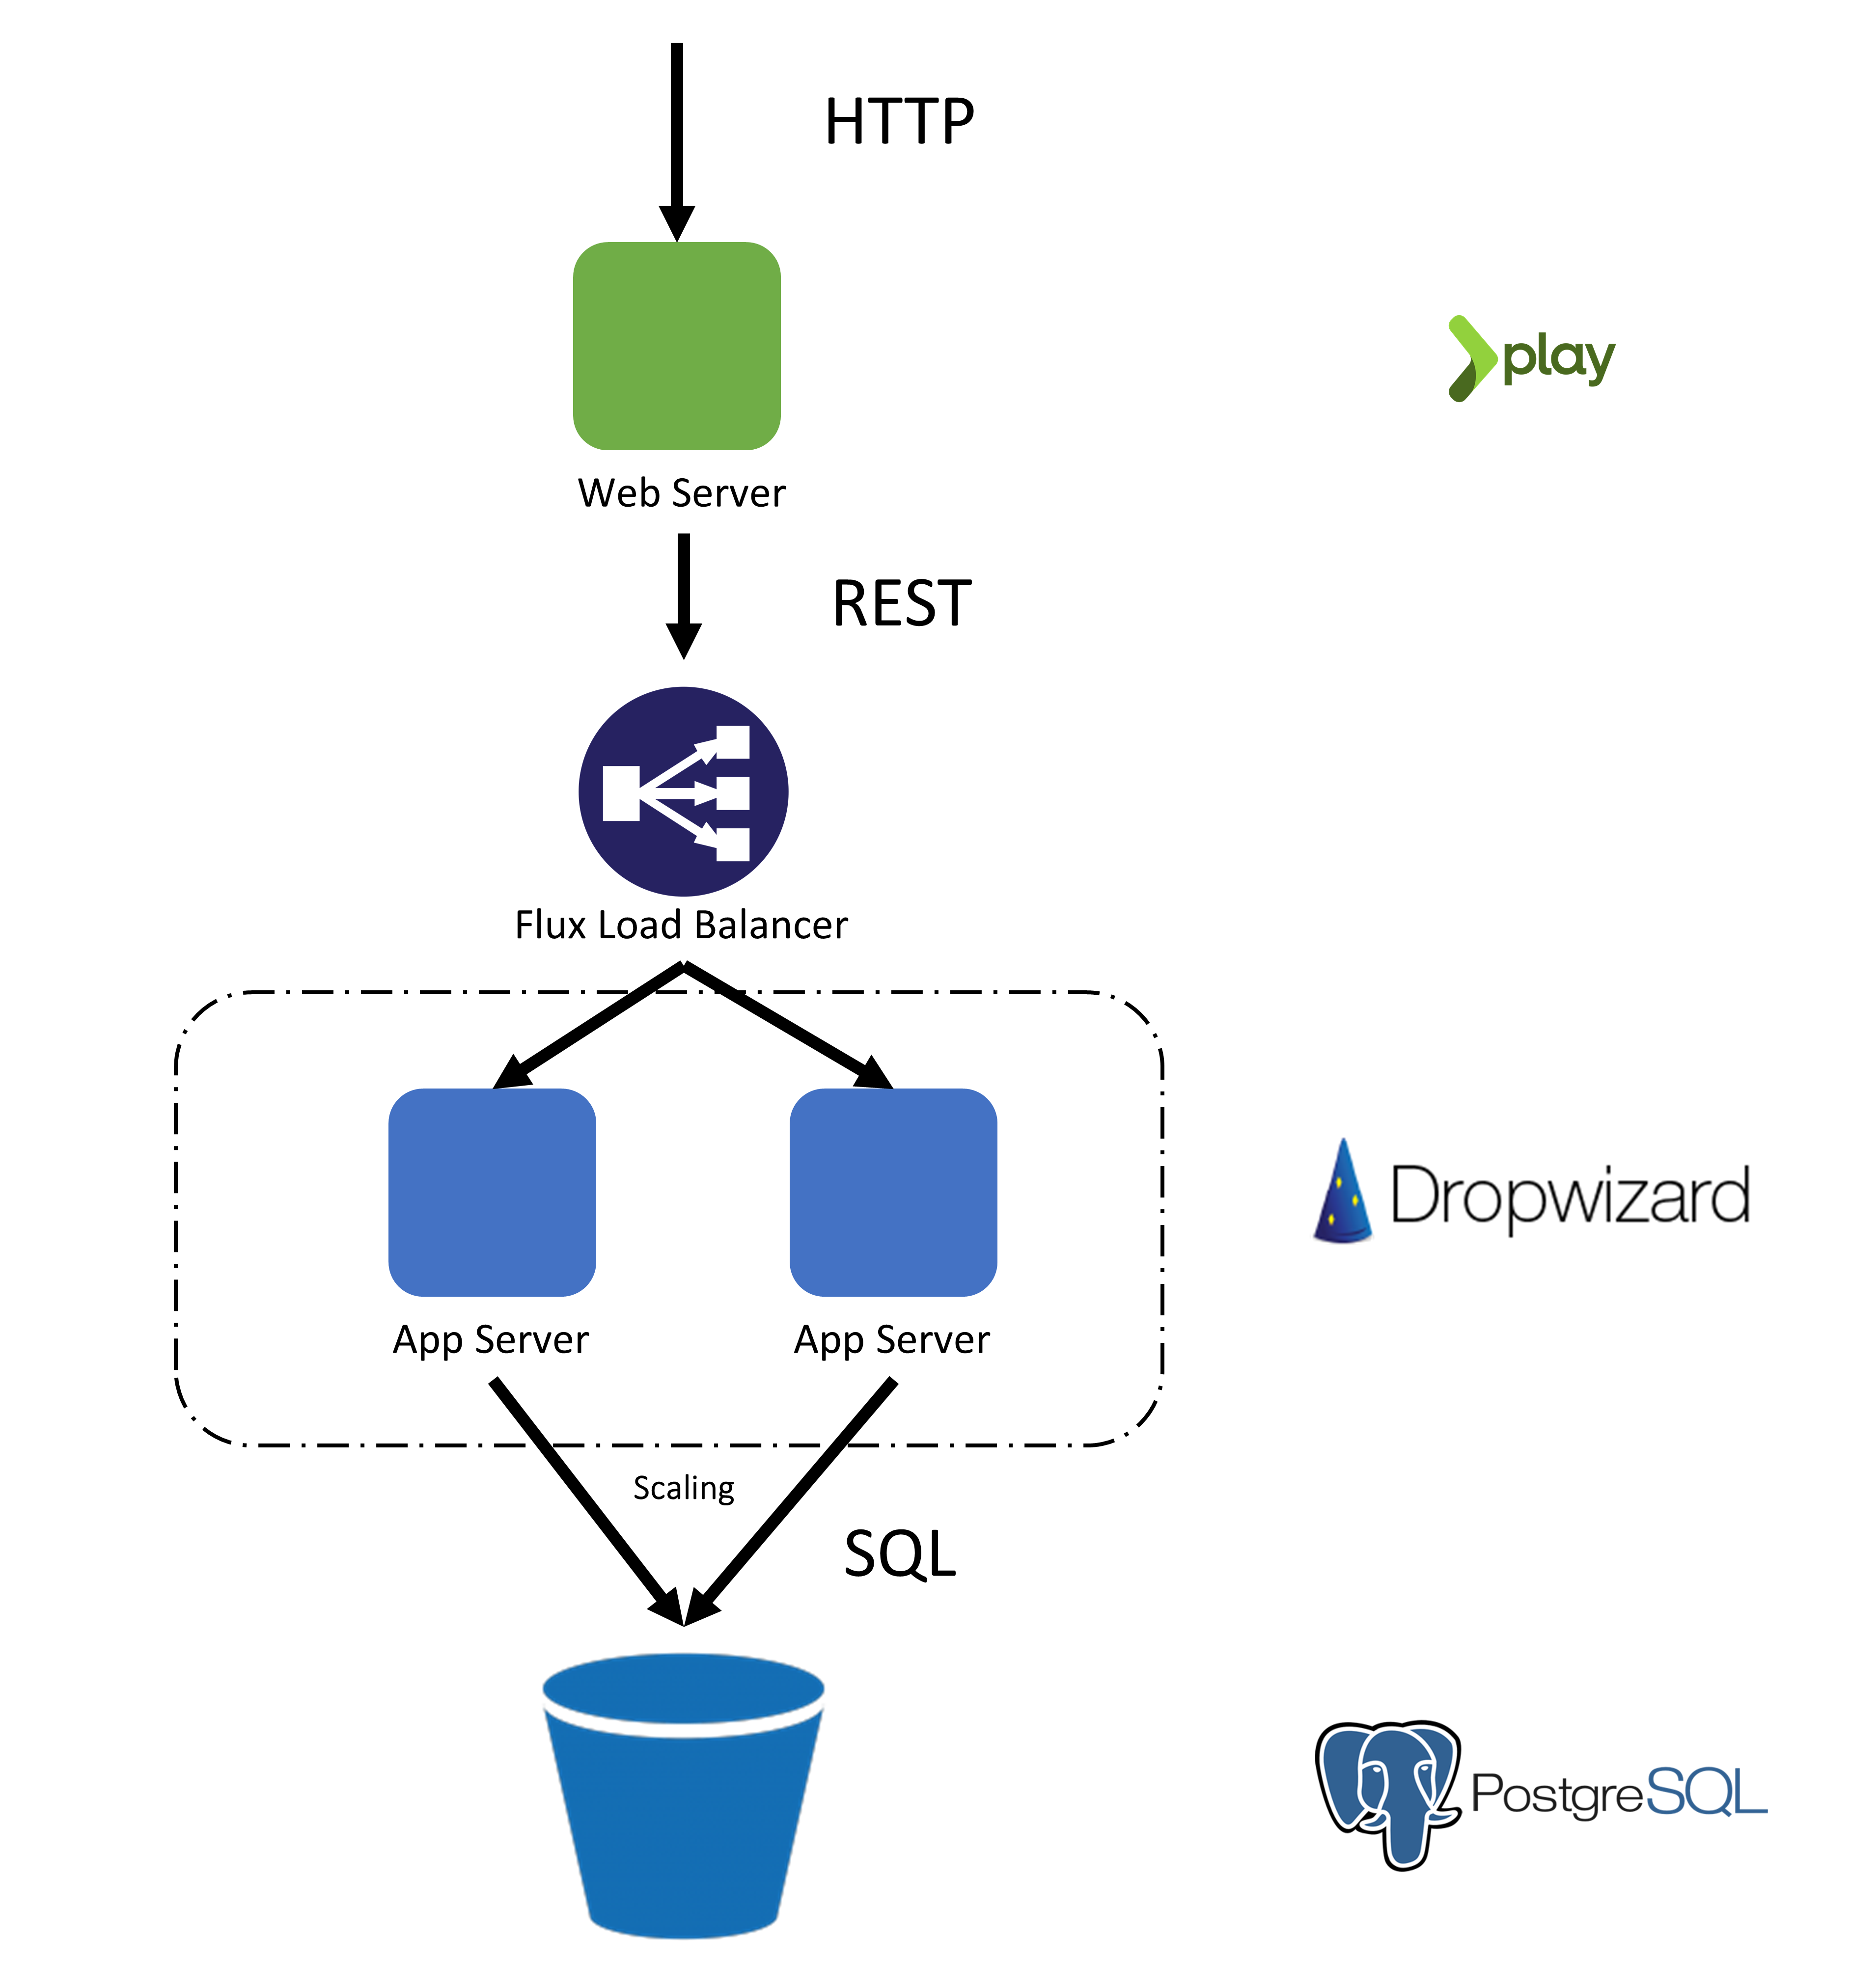
\includegraphics[height=7cm]{images/Architektur.png}
\caption{Tier des Verkehrsmodell-Fallstudien-Editor}
\label{tier_architecture}
\end{figure}
Durch die Anforderungen bezüglich Performance und Antwortgeschwindigkeiten musste die Architektur für die Softwarelösung des Verkehrsmodell-Fallstudien-Editor skalierbar aufgebaut werden. Eine Entkopplung der Komponenten erlaubt eine Verteilung und kann daher die Last auf dem einzelnen Server senken. Die Softwarelösung für den Verkehrsmodell-Fallstudien-Editor ist daher als 3-Tier Applikation aufgebaut. Der Frontside-Tier ist ein Webprojekt implementiert mit dem Play Framework. Der Backend-Tier wird als REST Service (Maturity Level 2) mit Dropwizard entwickelt. Der Daten-Tier wird durch eine PostgreSQL Datenbank bereitgestellt. Der Backend-Tier wird durch eine Load Balancer skalierbar und kann daher mehrere Anfragen parallel ausführen.\\
\section{SimMap-Editor}
TODO
\section{SimMap-Service}
TODO
\section{Datenbank}
TODO